% Paytm Hisaab -- demo-day pitch (19 Sep 2026)
% Paytm Build for India AI Hackathon, Bengaluru Edition. Track 3: Autonomous AI Teammates.
%
% A copy of ../proposal/hisaab-proposal.tex (Round 1), rewritten against what the bfi branch actually runs.
% Anything the prototype does not do yet is marked "next", never claimed. Legal claims follow
% legal/citations.yaml, including its deck_v2_corrections: the SOP is not cited for mule vs
% bona fide (the courts are), and "if the trail is verified" is gone.
%
% Compile with XeLaTeX or Tectonic (needed for the rupee sign), twice so the page total resolves:
%
%   cd pitch
%   xelatex hisaab-demo-day.tex && xelatex hisaab-demo-day.tex
%   tectonic hisaab-demo-day.tex
%
% Fonts: Segoe UI (Windows), else Helvetica Neue (macOS). Both carry the rupee sign.
\documentclass[aspectratio=169,10pt]{beamer}

\usepackage{fontspec}
\usepackage{amssymb}
\usepackage{tikz}
\usepackage{array}
\newcolumntype{L}[1]{>{\raggedright\arraybackslash}p{#1}}
\usetikzlibrary{calc,positioning,arrows.meta}

% ---------- team (fill in; left empty, nothing is printed) ----------
\def\teamname{}
\def\teammembers{}

% ---------- fonts ----------
\IfFontExistsTF{Segoe UI}{\setsansfont{Segoe UI}}{%
  \IfFontExistsTF{Helvetica Neue}{\setsansfont{Helvetica Neue}[
    BoldFont={Helvetica Neue Bold}, ItalicFont={Helvetica Neue Italic},
    BoldItalicFont={Helvetica Neue Bold Italic}]}{}}
\renewcommand{\familydefault}{\sfdefault}

\hyphenpenalty=10000
\exhyphenpenalty=10000
\emergencystretch=3em
\hbadness=10000

% ---------- palette ----------
\definecolor{navy}{HTML}{002970}
\definecolor{ptmcyan}{HTML}{00BAF2}
\definecolor{ink}{HTML}{0F172A}
\definecolor{muted}{HTML}{64748B}
\definecolor{good}{HTML}{15803D}
\definecolor{bad}{HTML}{DC2626}
\definecolor{amber}{HTML}{B45309}
\definecolor{tint}{HTML}{EAF4FD}
\definecolor{hairline}{HTML}{DBE7F3}

% ---------- theme ----------
\usetheme{default}
\usecolortheme{default}
\setbeamertemplate{navigation symbols}{}
\setbeamersize{text margin left=0.85cm,text margin right=0.85cm}
\setbeamercolor{normal text}{fg=ink,bg=white}
\setbeamercolor{frametitle}{fg=navy}
\setbeamercolor{structure}{fg=navy}
\setbeamerfont{frametitle}{size=\Large,series=\bfseries}

% the section label printed above every frame title
\def\secttag{}
\newcommand{\sect}[1]{\def\secttag{#1}}
\setbeamertemplate{frametitle}{%
  \vspace{0.25cm}%
  {\fontsize{7}{8}\selectfont\bfseries\color{ptmcyan}\secttag}\par\vspace{0.1em}%
  \usebeamerfont{frametitle}\usebeamercolor[fg]{frametitle}\insertframetitle\par\vspace{0.15em}%
  {\color{ptmcyan}\rule{1.2cm}{2pt}}\par\vspace{-0.2cm}%
}
\setbeamertemplate{footline}{%
  \hbox{\begin{beamercolorbox}[wd=\paperwidth,ht=1.9ex,dp=1.1ex,leftskip=0.85cm,rightskip=0.85cm]{}%
  {\scriptsize\color{muted}\hfill\insertframenumber\,/\,\inserttotalframenumber}%
  \end{beamercolorbox}}%
}

% ---------- helpers ----------
\newcommand{\hi}[1]{\leavevmode{\color{navy}\bfseries #1}}
\newcommand{\qm}[1]{``#1''}
\newcommand{\ok}{{\color{good}$\checkmark$}}
% a red label that starts a table cell (\leavevmode keeps it on the row's first line)
\newcommand{\wontcross}[1]{\leavevmode{\color{bad}\bfseries #1}}
% bullet and check with a hanging indent
\newcommand{\bpt}[1]{{\hangindent=0.9em\hangafter=1\noindent\makebox[0.9em][l]{\color{ptmcyan}\textbullet}#1\par}\vspace{0.3em}}
\newcommand{\chk}[1]{{\hangindent=1.4em\hangafter=1\noindent\makebox[1.4em][l]{\color{good}\large$\checkmark$}#1\par}\vspace{0.9em}}
% compact status lines: working today, or next
\newcommand{\done}[1]{{\hangindent=1.2em\hangafter=1\noindent\makebox[1.2em][l]{\color{good}$\checkmark$}#1\par}\vspace{0.28em}}
\newcommand{\todo}[1]{{\hangindent=1.2em\hangafter=1\noindent\makebox[1.2em][l]{\color{muted}$\circ$}{\color{muted}#1}\par}\vspace{0.28em}}
% \boxcard{fill}{draw}{width}{height or empty}{body}; top-aligned so cards in a row line up
\newcommand{\boxcard}[5]{%
  \begin{tikzpicture}[baseline=(current bounding box.north)]%
  \node[rounded corners=5pt,fill=#1,draw=#2,line width=1pt,inner sep=8pt,font=\small]{%
    \if\relax\detokenize{#4}\relax\begin{minipage}{#3}\else\begin{minipage}[t][#4][t]{#3}\fi
    \raggedright #5\end{minipage}};%
  \end{tikzpicture}}
\newcommand{\card}[3][]{\boxcard{tint}{none}{#2}{#1}{#3}}
\newcommand{\ocard}[4][]{\boxcard{white}{#2}{#3}{#1}{#4}}
\newcommand{\ncard}[3][]{\boxcard{navy}{none}{#2}{#1}{\color{white}#3}}
% big number:  \stat{colour}{number}{label}
\newcommand{\stat}[3]{\ocard{#1}{3.95cm}{\centering{\fontsize{28}{30}\selectfont\bfseries\color{#1}#2\par}\vspace{0.25em}{\color{muted}#3\par}}}
% heading + short line:  \tile{width}{height}{heading}{body}
\newcommand{\tile}[4]{\card[#2]{#1}{{\normalsize\bfseries\color{navy}#3\par}\vspace{0.3em}#4}}
% a workflow lane with a status on each step:  \slane{colour}{title}{\done or \todo lines}
\newcommand{\slane}[3]{\ocard[2.35cm]{#1}{3.95cm}{{\large\bfseries\color{#1}#2\par}\vspace{0.6em}#3}}

\tikzset{
  hbx/.style={rounded corners=4pt,fill=tint,inner sep=6pt,align=left,font=\footnotesize,text width=#1},
  flow/.style={-{Stealth[length=2.2mm]},ptmcyan,line width=1.3pt},
  flow2/.style={{Stealth[length=2.2mm]}-{Stealth[length=2.2mm]},ptmcyan,line width=1.3pt},
}

\begin{document}

% ============================================================ 1. TITLE
{\setbeamertemplate{footline}{}
\begin{frame}[plain]
\vspace{0.5cm}
\begin{center}
{\scriptsize\bfseries\color{ptmcyan}WORKING PROTOTYPE \;$\cdot$\; DEMO DAY, 19 SEPTEMBER 2026}\\[1em]
{\fontsize{40}{44}\selectfont\bfseries\color{navy}Paytm\;\color{ink}Hisaab}\\[0.5em]
{\Large\color{muted}Every rupee, on your side.}\\[1em]
{\color{ptmcyan}\rule{2.8cm}{2.5pt}}\\[1em]
{\large\color{ink}An AI teammate that explains a merchant's money}\\[0.2em]
{\large\color{ink}when a freeze or a tax notice hits.}\\[1.4em]
{\small\color{muted}Track 3: Autonomous AI Teammates \;$\cdot$\; Paytm Build for India AI Hackathon, Bengaluru}\\[0.45em]
{\scriptsize\color{muted}Built on n8n \;$\cdot$\; Sarvam AI \;$\cdot$\; Cognee \;$\cdot$\; PostgreSQL}
\ifx\teamname\empty\else\\[0.9em]{\small\bfseries\color{navy}Team \teamname}\fi
\ifx\teammembers\empty\else\\[0.2em]{\scriptsize\color{muted}\teammembers}\fi
\end{center}
\end{frame}}

% ============================================================ 2. PROBLEM: THE CONTEXT
\sect{PROBLEM STATEMENT}
\begin{frame}{Small merchants can't explain their own UPI money}
\vspace{0.35cm}
{\centering
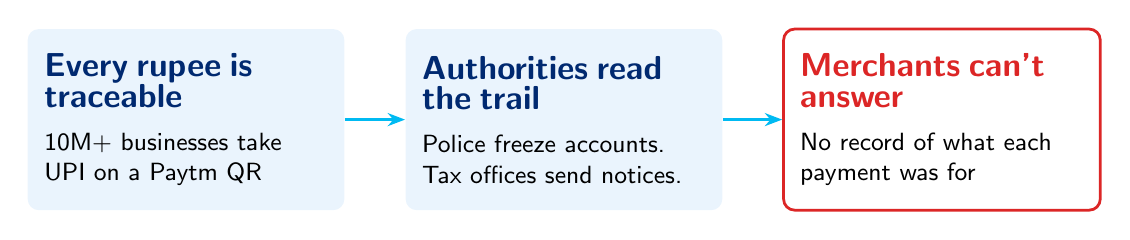
\begin{tikzpicture}
\tikzset{ctx/.style={hbx=3.6cm,minimum height=2.3cm,font=\small}}
\node[ctx] (a) at (0,0)
  {{\large\bfseries\color{navy}Every rupee is traceable}\\[0.5em]10M+ businesses take UPI on a Paytm QR};
\node[ctx] (b) at (4.8,0)
  {{\large\bfseries\color{navy}Authorities read the trail}\\[0.5em]Police freeze accounts. Tax offices send notices.};
\node[ctx,fill=white,draw=bad,line width=1pt] (c) at (9.6,0)
  {{\large\bfseries\color{bad}Merchants can't answer}\\[0.5em]No record of what each payment was for};
\draw[flow] (a) -- (b); \draw[flow] (b) -- (c);
\end{tikzpicture}\par}
\vspace{0.7cm}
{\centering\ncard{13.2cm}{\centering\normalsize The result: \textbf{frozen accounts, wrong tax bills, and shops going back to cash.}}\par}
\end{frame}

% ============================================================ 3. PROBLEM: A TYPICAL FREEZE
\sect{PROBLEM STATEMENT \;$\cdot$\; A TYPICAL CASE}
\begin{frame}{One payment can freeze a whole shop}
\vspace{0.2cm}
\noindent\stat{bad}{₹4,200}{the disputed payment}\hfill
\stat{navy}{339}{payments that week}\hfill
\stat{bad}{100\%}{of the account frozen}
\par\vspace{0.5cm}
{\centering\small They sold onions to a customer three hops from a fraud. They aren't even named in the FIR.\par}
\vspace{0.45cm}
\noindent\card{3.95cm}{{\bfseries\color{navy}The bank}\par has no bill}\hfill
\card{3.95cm}{{\bfseries\color{navy}The police officer}\par is in another state}\hfill
\card{3.95cm}{{\bfseries\color{navy}The merchant}\par can't find the payment}
\par\vspace{0.4cm}
{\centering\normalsize\hi{Nobody can say which payment it was, or what it paid for.}\par}
\end{frame}

% ============================================================ 4. PROBLEM: TWO AUTHORITIES
\sect{PROBLEM STATEMENT}
\begin{frame}{Two authorities now demand an answer}
\vspace{0.2cm}
\noindent\card[3.45cm]{6.4cm}{{\large\bfseries\color{bad}Cyber-crime freezes\par}
  {\footnotesize\color{muted}MHA/I4C SOP of 2 January 2026, and the High Courts\par}\vspace{0.5em}
  \bpt{Hold only the disputed amount, not the whole account}
  \bpt{\qm{Mule account} is a label, not a reason}
  \bpt{A shop can't check who is paying it by UPI}
  \vspace{0.05em}{\fontsize{6.5}{7.8}\selectfont\color{muted}Shree Balaji Enterprises v. RBI (Rajasthan HC, 20 Aug 2026); Sri Sai Wines v. Union of India (AP HC, 22 Jun 2026); Ritesh Yadav v. RBI (Allahabad HC, 14 Aug 2026)\par}}\hfill
\card[3.45cm]{6.4cm}{{\large\bfseries\color{amber}GST notices\par}
  {\footnotesize\color{muted}Haveri, Karnataka, 2025\par}\vspace{0.4em}
  {\centering{\fontsize{30}{32}\selectfont\bfseries\color{bad}₹29 lakh\par}}\vspace{0.4em}
  demanded from a vegetable seller whose sales were tax-exempt\par\vspace{0.4em}
  {\footnotesize\color{muted}Exempt sales still count toward turnover (CGST s.2(6)), so the answer needs the real split.\par}}
\par\vspace{0.4cm}
{\centering\ncard{13.2cm}{\centering\normalsize Both ask one question: \textbf{what was each rupee, actually?}}\par}
\end{frame}

% ============================================================ 5. SOLUTION: ONE LEDGER
\sect{PROPOSED SOLUTION}
\begin{frame}{One ledger, two answers}
\vspace{0.3cm}
{\centering
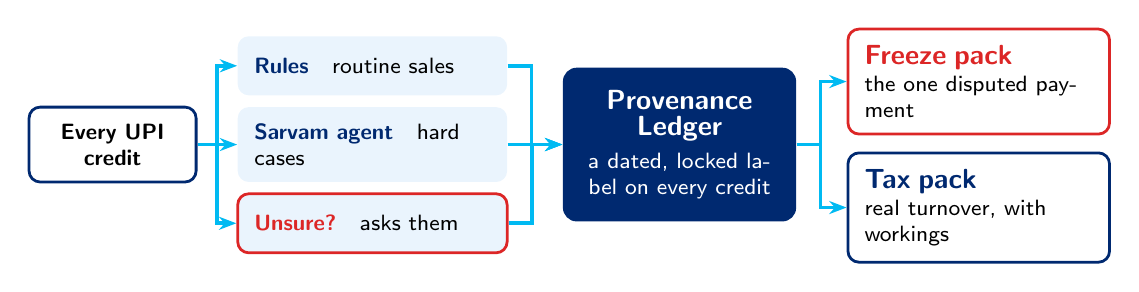
\begin{tikzpicture}
\node[hbx=1.7cm,fill=white,draw=navy,line width=1pt,align=center,font=\footnotesize\bfseries] (src) at (0,0) {Every UPI credit};
\node[hbx=3.0cm,minimum height=0.75cm] (rules) at (3.3,1.0)  {{\bfseries\color{navy}Rules}\quad routine sales};
\node[hbx=3.0cm,minimum height=0.75cm] (ai)    at (3.3,0)    {{\bfseries\color{navy}Sarvam agent}\quad hard cases};
\node[hbx=3.0cm,minimum height=0.75cm,draw=bad,line width=1pt] (ask) at (3.3,-1.0) {{\bfseries\color{bad}Unsure?}\quad asks them};
\node[rounded corners=5pt,fill=navy,text=white,inner sep=8pt,align=center,text width=2.4cm,font=\footnotesize] (led) at (7.2,0)
  {{\normalsize\bfseries Provenance Ledger}\\[0.3em]a dated, locked label on every credit};
\node[hbx=2.9cm,fill=white,draw=bad,line width=1pt] (o1) at (11.0,0.8)
  {{\normalsize\bfseries\color{bad}Freeze pack}\\the one disputed payment};
\node[hbx=2.9cm,fill=white,draw=navy,line width=1pt] (o2) at (11.0,-0.8)
  {{\normalsize\bfseries\color{navy}Tax pack}\\real turnover, with workings};
\foreach \n in {rules,ai,ask} {
  \draw[flow] (src.east) -- ++(0.25,0) |- (\n.west);
  \draw[flow] (\n.east) -- ++(0.3,0) |- (led.west);
}
\draw[flow] (led.east) -- ++(0.3,0) |- (o1.west);
\draw[flow] (led.east) -- ++(0.3,0) |- (o2.west);
\end{tikzpicture}\par}
\vspace{0.75cm}
{\centering\normalsize It never guesses: \hi{at most 3 questions a day}, one tap each, in their own language.\par}
\end{frame}

% ============================================================ 6. SOLUTION: END TO END, WITH STATUS
\sect{PROPOSED SOLUTION}
\begin{frame}{The teammate works each case end to end}
\vspace{0.2cm}
\noindent\slane{navy}{Every night}{\done{Labels new payments}\done{Asks up to 3 questions}\todo{Warns on WhatsApp before the GST limit}}\hfill
\slane{bad}{Account frozen}{\done{Finds the one payment}\done{Builds the evidence pack}\todo{Drafts the grievance}}\hfill
\slane{amber}{Tax notice}{\todo{Reads the notice photo}\done{Rebuilds real turnover}\todo{Explains it to their CA}}
\par\vspace{0.12cm}
{\raggedleft\scriptsize\color{muted}\ok\ runs in today's demo \quad {\color{muted}$\circ$} next\par}
\vspace{0.3cm}
\noindent\card{13.6cm}{{\bfseries\color{bad}Hands to a human} when the amount is large, the evidence is weak, the payment isn't a sale, or they dispute a label: seven rules, each with its reason.\par\vspace{0.25em}
{\bfseries\color{navy}Nothing is sent without a Paytm officer's approval, and the server enforces it.}}
\end{frame}

% ============================================================ 7. SOLUTION: TRACK 3 FIT
\sect{PROPOSED SOLUTION}
\begin{frame}{A teammate, not a chatbot}
\vspace{0.05cm}
{\normalsize\bfseries\color{ink}It understands, decides, acts, and knows when to hand over\par}
\vspace{0.35cm}
\noindent\tile{3.95cm}{1.45cm}{Understands context}{Each payer's history as of that payment, plus memory of the shop}\hfill
\tile{3.95cm}{1.45cm}{Makes decisions}{Picks 1 payment out of 339, and 3 questions out of 68}\hfill
\tile{3.95cm}{1.45cm}{Takes actions}{Opens the case, builds a fingerprinted evidence pack}
\par\vspace{0.3cm}
\noindent\tile{3.95cm}{1.45cm}{Works with humans}{They answer by tap or WhatsApp; an officer approves}\hfill
\tile{3.95cm}{1.45cm}{Escalates wisely}{Seven escalation rules, each with a written reason}\hfill
\tile{3.95cm}{1.45cm}{Measurable outcomes}{Freeze to pack to approval, timed by the server}
\end{frame}

% ============================================================ 8. DEMO: AN ORDINARY NIGHT
\sect{WORKING TODAY \;$\cdot$\; AN ORDINARY NIGHT}
\begin{frame}{68 payments in, 3 questions out}
\vspace{0.3cm}
{\centering
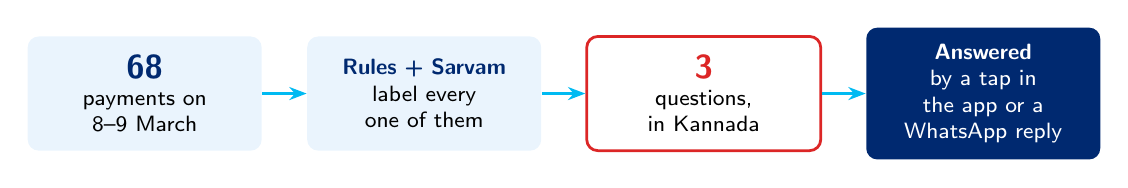
\begin{tikzpicture}
\tikzset{stp/.style={hbx=2.55cm,align=center,minimum height=1.45cm}}
\node[stp] (s1) at (0,0)     {{\large\bfseries\color{navy}68}\\payments on 8--9 March};
\node[stp] (s2) at (3.55,0)  {{\bfseries\color{navy}Rules + Sarvam}\\label every one of them};
\node[stp,fill=white,draw=bad,line width=1pt] (s3) at (7.1,0) {{\large\bfseries\color{bad}3}\\questions, in Kannada};
\node[stp,fill=navy,text=white] (s4) at (10.65,0) {{\bfseries Answered}\\by a tap in the app or a WhatsApp reply};
\draw[flow] (s1) -- (s2); \draw[flow] (s2) -- (s3); \draw[flow] (s3) -- (s4);
\end{tikzpicture}\par}
\vspace{0.45cm}
\noindent\ocard[1.75cm]{hairline}{3.95cm}{{\large\bfseries\color{navy}₹15,000\par}\vspace{0.2em}{\color{muted}late at night, from their linked savings account\par}\vspace{0.3em}Their answer: \textbf{own money}}\hfill
\ocard[1.75cm]{hairline}{3.95cm}{{\large\bfseries\color{navy}₹7,500\par}\vspace{0.2em}{\color{muted}their spouse, scanned at the shop QR\par}\vspace{0.3em}Their answer: \textbf{family}}\hfill
\ocard[1.75cm]{hairline}{3.95cm}{{\large\bfseries\color{navy}₹4,850\par}\vspace{0.2em}{\color{muted}a customer with only two earlier purchases\par}\vspace{0.3em}Their answer: \textbf{a sale}}
\par\vspace{0.4cm}
{\centering\small The other 65 are labelled without asking, the ₹23 one included. \hi{The AI's label stays beside their answer, both dated.}\par}
\end{frame}

% ============================================================ 9. DEMO: THE FREEZE
\sect{WORKING TODAY \;$\cdot$\; THE FREEZE}
\begin{frame}{From a lien to an approved pack}
\vspace{0.25cm}
{\centering
\begin{tikzpicture}
\tikzset{stp/.style={hbx=2.1cm,align=left,minimum height=2.35cm,font=\scriptsize}}
\node[stp] (s1) at (0,0)
  {{\normalsize\bfseries\color{navy}1\;Lien}\\[0.3em]24 Mar, 09:30.\\The case opens by itself.};
\node[stp] (s2) at (2.85,0)
  {{\normalsize\bfseries\color{navy}2\;Isolate}\\[0.3em]₹4,200 on 21 Mar at 19:47\\[0.2em]\ok\ by UTR\\\ok\ by amount + date};
\node[stp,fill=white,draw=amber,line width=1pt] (s3) at (5.7,0)
  {{\normalsize\bfseries\color{amber}3\;Decoy}\\[0.3em]₹4,200 on 18 Mar from a regular.\\Listed, \textbf{not chosen}.};
\node[stp] (s4) at (8.55,0)
  {{\normalsize\bfseries\color{navy}4\;Pack}\\[0.3em]The bill, the till, 1 of 339.\\Tier 1. PDF fingerprinted.};
\node[stp,fill=navy,text=white] (s5) at (11.4,0)
  {{\normalsize\bfseries 5\;Approve}\\[0.3em]Officer approves on their phone. Sent (simulated).};
\draw[flow] (s1) -- (s2); \draw[flow] (s2) -- (s3); \draw[flow] (s3) -- (s4); \draw[flow] (s4) -- (s5);
\end{tikzpicture}\par}
\vspace{0.35cm}
\noindent\stat{navy}{1 of 339}{credits that week}\hfill
\stat{good}{2}{independent matches}\hfill
\stat{bad}{0}{sends before approval}
\par\vspace{0.25cm}
{\centering\small A send before approval is refused by the server. The merchant's case tracker moves to \qm{sent}.\par}
\end{frame}

% ============================================================ 10. SOLUTION: TRUST
\sect{PROPOSED SOLUTION}
\begin{frame}{A record nobody can fake later}
\vspace{0.25cm}
\begin{columns}[T]
\begin{column}{0.43\textwidth}
\vspace{0.35cm}
{\normalsize
\chk{Append-only and hash-chained, per shop}
\chk{The database refuses edits and deletes}
\chk{Their answers never overwrite the AI's label}
\chk{The database stamps the time, so nobody can backdate}}
\end{column}
\begin{column}{0.53\textwidth}
{\normalsize\bfseries\color{navy}Every line of the pack is graded\par}\vspace{0.5em}
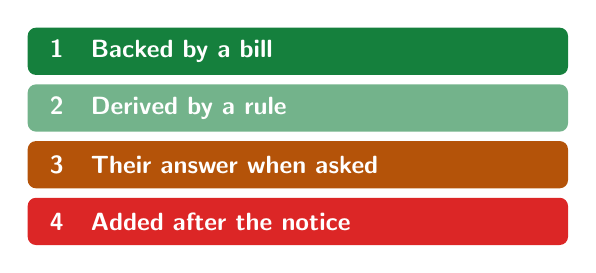
\begin{tikzpicture}
\foreach \c/\t [count=\k] in {good/Backed by a bill, good!60/Derived by a rule, amber/Their answer when asked, bad/Added after the notice} {
  \node[fill=\c,text=white,rounded corners=3pt,text width=6.3cm,minimum height=0.6cm,align=left,anchor=north west,inner xsep=8pt,font=\small\bfseries]
    at (0,-0.72*\k) {\k\quad\t};
}
\end{tikzpicture}\par\vspace{0.4em}
{\small\color{muted}Each pack reports the share held in tiers 1 and 2: a history made up after the fact can't fill them.\par}
\end{column}
\end{columns}
\vspace{0.55cm}
{\centering\large\hi{We sort. We don't advocate.}\par}
\end{frame}

% ============================================================ 11. LINES WE WON'T CROSS
\sect{PROPOSED SOLUTION}
\begin{frame}{Lines we won't cross, enforced in code}
\vspace{0.35cm}
{\small
\renewcommand{\arraystretch}{1.5}
\begin{tabular}{@{}L{4.3cm}L{9.2cm}@{}}
\wontcross{Never claims innocence} & A guard rejects any draft that asserts it as fact \\
\wontcross{Nothing sent unapproved} & The server refuses a send without an officer's approval in the ledger \\
\wontcross{The AI never does the maths} & A guard rejects any figure that Python didn't compute \\
\wontcross{Only verified law} & 10 sources checked by hand; an unverified one blocks approval \\
\wontcross{Never helps dodge tax} & Every turnover answer carries the registration verdict \\
\end{tabular}}
\par\vspace{0.4cm}
{\centering\ncard{13.2cm}{\centering\normalsize The guards are plain Python, not prompts. \textbf{If a check can't decide, it fails closed.}}\par}
\end{frame}

% ============================================================ 12. TECH: ARCHITECTURE AS BUILT
\sect{TECHNOLOGY STACK}
\begin{frame}{Architecture, as built}
\vspace{0.05cm}
{\centering
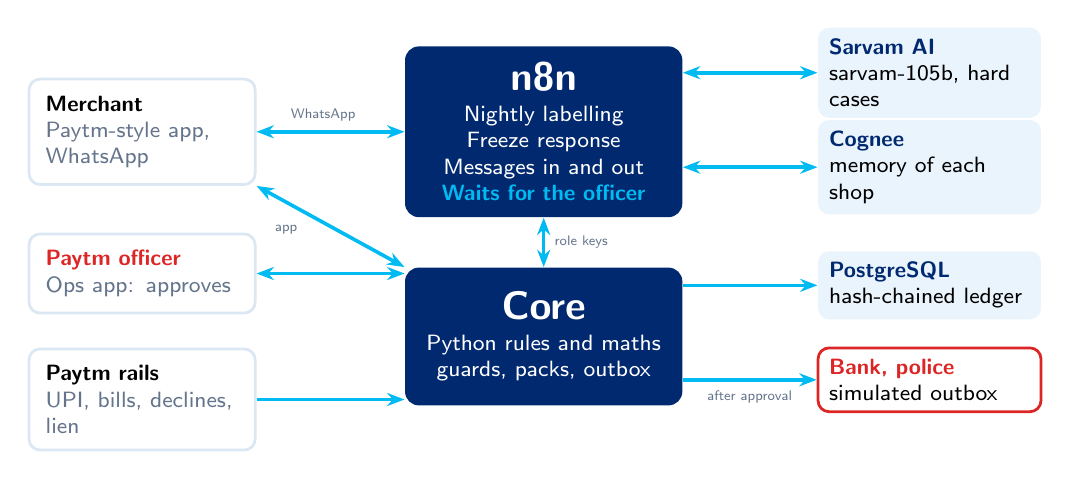
\begin{tikzpicture}
\tikzset{
  actor/.style={hbx=2.45cm,fill=white,draw=hairline,line width=1pt},
  svc/.style={hbx=2.55cm,inner sep=4pt},
  big/.style={rounded corners=5pt,fill=navy,text=white,inner sep=6pt,align=center,text width=3.1cm,font=\footnotesize},
}
\node[actor] (mer)   at (0,1.2)   {{\bfseries Merchant}\\{\color{muted}Paytm-style app, WhatsApp}};
\node[actor] (off)   at (0,-0.6) {{\bfseries\color{bad}Paytm officer}\\{\color{muted}Ops app: approves}};
\node[actor] (rails) at (0,-2.2)  {{\bfseries Paytm rails}\\{\color{muted}UPI, bills, declines, lien}};
\node[big,minimum height=2.05cm] (n8n) at (5.1,1.2)
  {{\Large\bfseries n8n}\\[0.2em]Nightly labelling\\Freeze response\\Messages in and out\\{\color{ptmcyan}\bfseries Waits for the officer}};
\node[big,minimum height=1.75cm] (core) at (5.1,-1.4)
  {{\Large\bfseries Core}\\[0.2em]Python rules and maths\\guards, packs, outbox};
\node[svc] (sar) at (10.0,1.95)  {{\bfseries\color{navy}Sarvam AI}\\sarvam-105b, hard cases};
\node[svc] (cog) at (10.0,0.75)  {{\bfseries\color{navy}Cognee}\\memory of each shop};
\node[svc] (db)  at (10.0,-0.75) {{\bfseries\color{navy}PostgreSQL}\\hash-chained ledger};
\node[svc,fill=white,draw=bad,line width=1pt] (out) at (10.0,-1.95) {{\bfseries\color{bad}Bank, police}\\simulated outbox};
\draw[flow2] (mer.east) -- node[above,font=\tiny,color=muted,pos=0.45]{WhatsApp} (mer.east -| n8n.west);
\draw[flow2] (mer.south east) -- node[below left,font=\tiny,color=muted,pos=0.35]{app} (core.north west);
\draw[flow2] (off.east) -- (core.west |- off.east);
\draw[flow]  (rails.east) -- (rails.east -| core.west);
\draw[flow2] (n8n.south) -- node[right,font=\tiny,color=muted]{role keys} (core.north);
\draw[flow2] (n8n.east |- sar.west) -- (sar.west);
\draw[flow2] (n8n.east |- cog.west) -- (cog.west);
\draw[flow]  (core.east |- db.west) -- (db.west);
\draw[flow]  (core.east |- out.west) -- node[below,font=\tiny,color=muted]{after approval} (out.west);
\end{tikzpicture}\par}
\vspace{0.2cm}
{\centering\small Every agent step is an n8n node you can open. \hi{Core, not the workflow, decides what may be written or sent.}\par}
\end{frame}

% ============================================================ 13. TECH STACK
\sect{TECHNOLOGY STACK}
\begin{frame}{Built on n8n, Sarvam AI and Cognee}
\vspace{0.2cm}
\noindent\tile{3.95cm}{1.1cm}{\large n8n}{{\color{muted}five workflows, one waits for a person}}\hfill
\tile{3.95cm}{1.1cm}{\large Sarvam AI}{{\color{muted}sarvam-105b labels the hard cases}}\hfill
\tile{3.95cm}{1.1cm}{\large Cognee}{{\color{muted}a separate memory for each shop}}
\par\vspace{0.3cm}
\noindent\tile{3.95cm}{1.1cm}{\large Python + FastAPI}{{\color{muted}rules, maths, guards, PDF packs}}\hfill
\tile{3.95cm}{1.1cm}{\large PostgreSQL}{{\color{muted}an append-only, hash-chained ledger}}\hfill
\tile{3.95cm}{1.1cm}{\large WhatsApp + app}{{\color{muted}Kannada, Hindi and English}}
\par\vspace{0.55cm}
{\centering

\begin{tikzpicture}[font=\small]
\node[hbx=2.6cm,align=center] (a) at (0,0)    {\bfseries AI proposes};
\node[hbx=2.6cm,align=center] (b) at (3.6,0)  {\bfseries Python calculates};
\node[hbx=2.6cm,align=center] (c) at (7.2,0)  {\bfseries Ledger records};
\node[hbx=2.6cm,align=center,fill=navy,text=white] (d) at (10.8,0) {\bfseries A person approves};
\draw[flow] (a) -- (b); \draw[flow] (b) -- (c); \draw[flow] (c) -- (d);
\end{tikzpicture}\par}
\end{frame}

% ============================================================ 14. USP
\sect{USP}
\begin{frame}{Why only Paytm can do this}
\vspace{0.2cm}
\noindent\tile{6.4cm}{1.45cm}{\large 1\;\; On the rail}{Sees every payment the moment it moves\par\vspace{0.15em}{\footnotesize\color{muted}Khatabook, Vyapar and ClearTax work after the fact}}\hfill
\tile{6.4cm}{1.45cm}{\large 2\;\; Two authorities, one engine}{Police and tax answered from one ledger\par\vspace{0.15em}{\footnotesize\color{muted}Other tools do one or the other}}
\par\vspace{0.3cm}
\noindent\tile{6.4cm}{1.45cm}{\large 3\;\; Can't be faked later}{Hash-chained from the day each payment lands\par\vspace{0.15em}{\footnotesize\color{muted}A mule can't backdate a clean history}}\hfill
\tile{6.4cm}{1.45cm}{\large 4\;\; Already the channel}{Paytm already answers banks and police\par\vspace{0.15em}{\footnotesize\color{muted}They confirm; Paytm responds in time}}
\par\vspace{0.5cm}
{\centering\normalsize\hi{Why now:} CFCFRMS opened a freeze-grievance module in April 2026, and High Courts have ruled a lien should cover only the disputed amount.\par}
\end{frame}

% ============================================================ 15. IMPACT
\sect{IMPACT \& BENEFITS}
\begin{frame}{Everyone in the loop wins}
\vspace{0.25cm}
\begin{columns}[T]
\begin{column}{0.31\textwidth}
\ncard[3.4cm]{3.5cm}{\centering\vfill{\fontsize{36}{38}\selectfont\bfseries 10M+\par}\vspace{0.5em}{\small businesses on a Paytm business QR could use it\par}\vfill}
\end{column}
\begin{column}{0.65\textwidth}
{\normalsize
\begin{tabular}{@{}L{2.6cm}L{6.3cm}@{}}
\hi{Merchant} & Keeps trading: only the disputed amount is held \\ \noalign{\vspace{0.75em}}
\hi{Paytm} & Keeps the GMV, the Soundbox and the loans \\ \noalign{\vspace{0.75em}}
\hi{Banks, police} & Get a verified trail they can act on \\ \noalign{\vspace{0.75em}}
\hi{UPI economy} & Fewer \qm{No UPI, cash only} signs \\
\end{tabular}}
\end{column}
\end{columns}
\vspace{0.45cm}
{\centering\footnotesize\color{muted}32.80 lakh cyber-fraud complaints on CFCFRMS, and 32.08 lakh Layer-1 mule accounts flagged, to 30 June 2026 (PIB)\par}
\vspace{0.2cm}
{\centering\small\color{muted}In a pilot we measure: days to release \;$\cdot$\; balance kept usable \;$\cdot$\; merchants still active after 30 days\par}
\end{frame}

% ============================================================ 16. BUSINESS MODEL
\sect{BUSINESS MODEL}
\begin{frame}{Business model}
\vspace{0.2cm}
\noindent\tile{6.4cm}{1.15cm}{\large Retention\hfill{\footnotesize\color{muted}\mdseries Paytm pays}}{Frozen merchants stay and keep transacting}\hfill
\tile{6.4cm}{1.15cm}{\large Hisaab Pro\hfill{\footnotesize\color{muted}\mdseries Merchant pays}}{A monthly add-on to their Soundbox plan}
\par\vspace{0.3cm}
\noindent\tile{6.4cm}{1.15cm}{\large Credit\hfill{\footnotesize\color{muted}\mdseries Lenders pay}}{Documented turnover unlocks loans}\hfill
\tile{6.4cm}{1.15cm}{\large Verification\hfill{\footnotesize\color{muted}\mdseries Banks pay}}{Checks whether a receiver is a genuine seller}
\par\vspace{0.55cm}
{\centering\ncard{10.5cm}{\centering\normalsize\bfseries Never charged: getting your own money released.}\par}
\end{frame}

% ============================================================ 17. BUILT AND NEXT
\sect{WHERE WE ARE}
\begin{frame}{Built in two days, and what comes next}
\vspace{0.15cm}
\noindent\ocard[3.75cm]{good}{6.45cm}{{\large\bfseries\color{good}Working in the demo\par}\vspace{0.4em}\footnotesize
\done{A hash-chained ledger that refuses edits}
\done{Nightly labelling, with 3 questions in Kannada}
\done{Answers by app tap or WhatsApp reply}
\done{Freeze: case, isolation, fingerprinted PDF pack}
\done{Officer approval before a simulated send}
\done{Tiers, guards, turnover, threshold, escalation}
\done{Merchant and officer apps in 3 languages}
\done{A demo reset in 36 seconds}}\hfill
\ocard[3.75cm]{hairline}{6.45cm}{{\large\bfseries\color{navy}Next\par}\vspace{0.4em}\footnotesize
\todo{A grievance drafted only from verified law}
\todo{A notice photo read by Sarvam Vision, then the tax pack}
\todo{The threshold warning on WhatsApp}
\todo{Voice notes, in and out}
\todo{A daily fingerprint anchored outside Paytm}
\todo{A full year labelled, so turnover covers every payment}
\todo{The same workflows running on n8n Cloud}}
\par\vspace{0.25cm}
{\centering\scriptsize\color{muted}All data is synthetic: every person, shop and case is fictional. Sends to banks and police are simulated.\par}
\vspace{0.15cm}
{\centering{\large\color{navy}\bfseries Paytm Hisaab}\quad{\color{muted}every rupee, on your side.}\par}
\end{frame}

\end{document}
